\documentclass[]{article}
\usepackage[utf8]{inputenc}
\usepackage{polski}
\usepackage{graphicx}
\graphicspath{ {./images/} }
\usepackage[margin=0.5in]{geometry}
\usepackage{gensymb}
\usepackage{textcomp}
\usepackage{siunitx}
\usepackage{float}
\documentclass{article}
\usepackage{graphicx}
\usepackage{wrapfig}
\usepackage{lipsum}
\usepackage{graphicx}
\usepackage{subcaption}


\begin{document}

\begin{figure}[tp!]
	\center{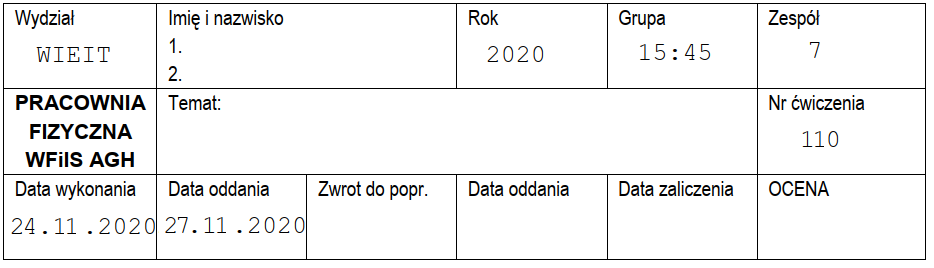
\includegraphics{F}}
\end{figure}

\begin{center}
	\section*{Sprawność urządzeń technicznych }
	\emph{Dzmitry Mikialevich}
\end{center}
\begin{center}
	\emph{Wojciech Sikora}
\end{center}
\tableofcontents
\newpage

\section{Wstęp}

\subsection{Cel ćwiczenia}
Wyznaczenie sprawności czajnika elektrycznego o znanej mocy znamionowej.

    


    
\section{Układ Pomiarowy}
W skład układu pomiarowego weszły następujące elementy:
\newline

1. Czajnik elektryczny


2. Termometr


3. Woda o znanej objętości

4. Stoper w smartfonie



\begin{figure}[H]
  \centering
  \begin{subfigure}[b]{0.4\linewidth}
    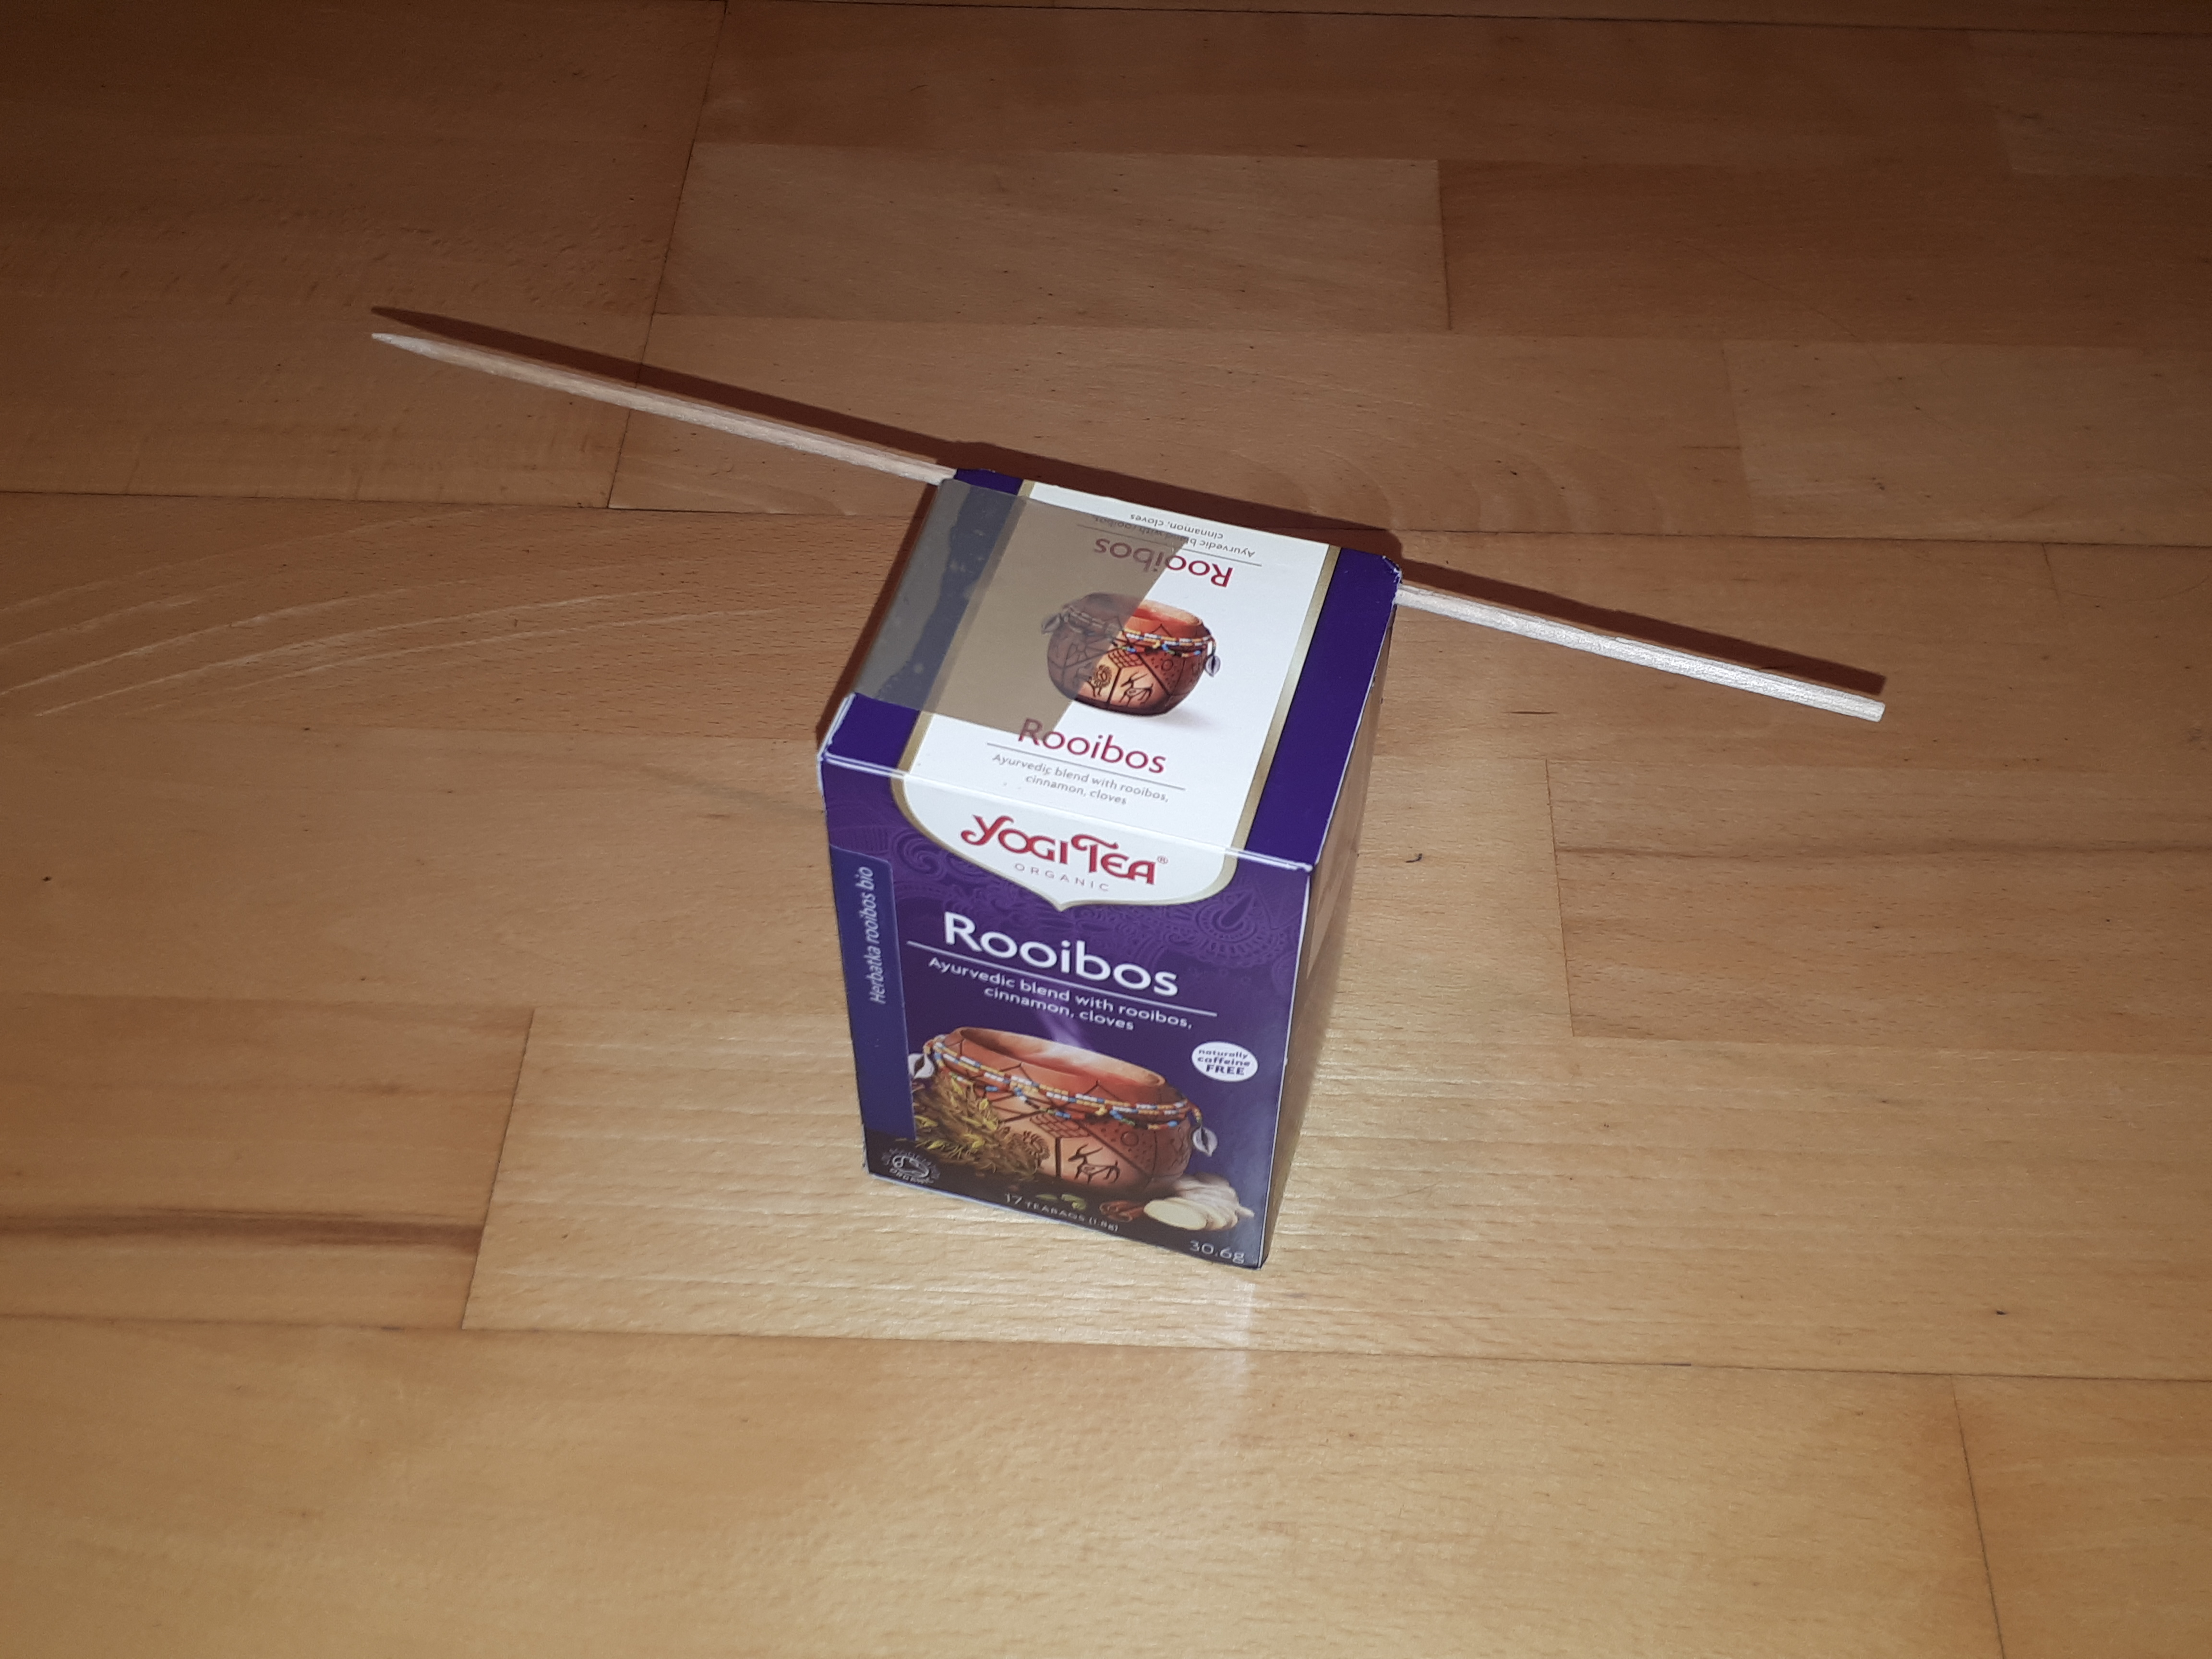
\includegraphics[width=\linewidth]{1}
    \caption{Szklanka z olejem}
  \end{subfigure}
  \begin{subfigure}[b]{0.4\linewidth}
    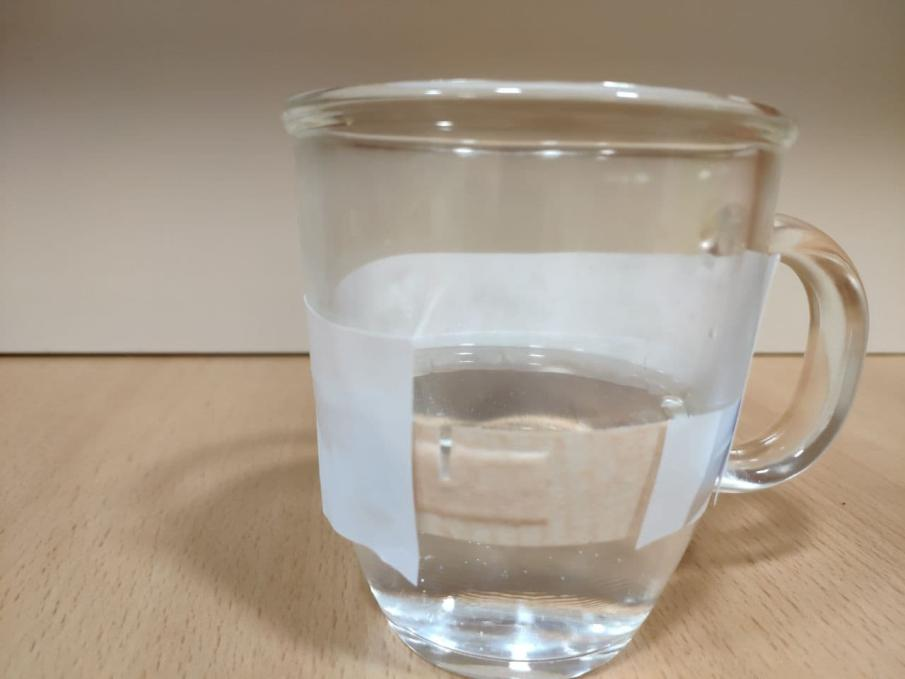
\includegraphics[width=\linewidth]{2}
    \caption{Szklanka z wodą}
  \end{subfigure}
  \begin{subfigure}[b]{0.4\linewidth}
    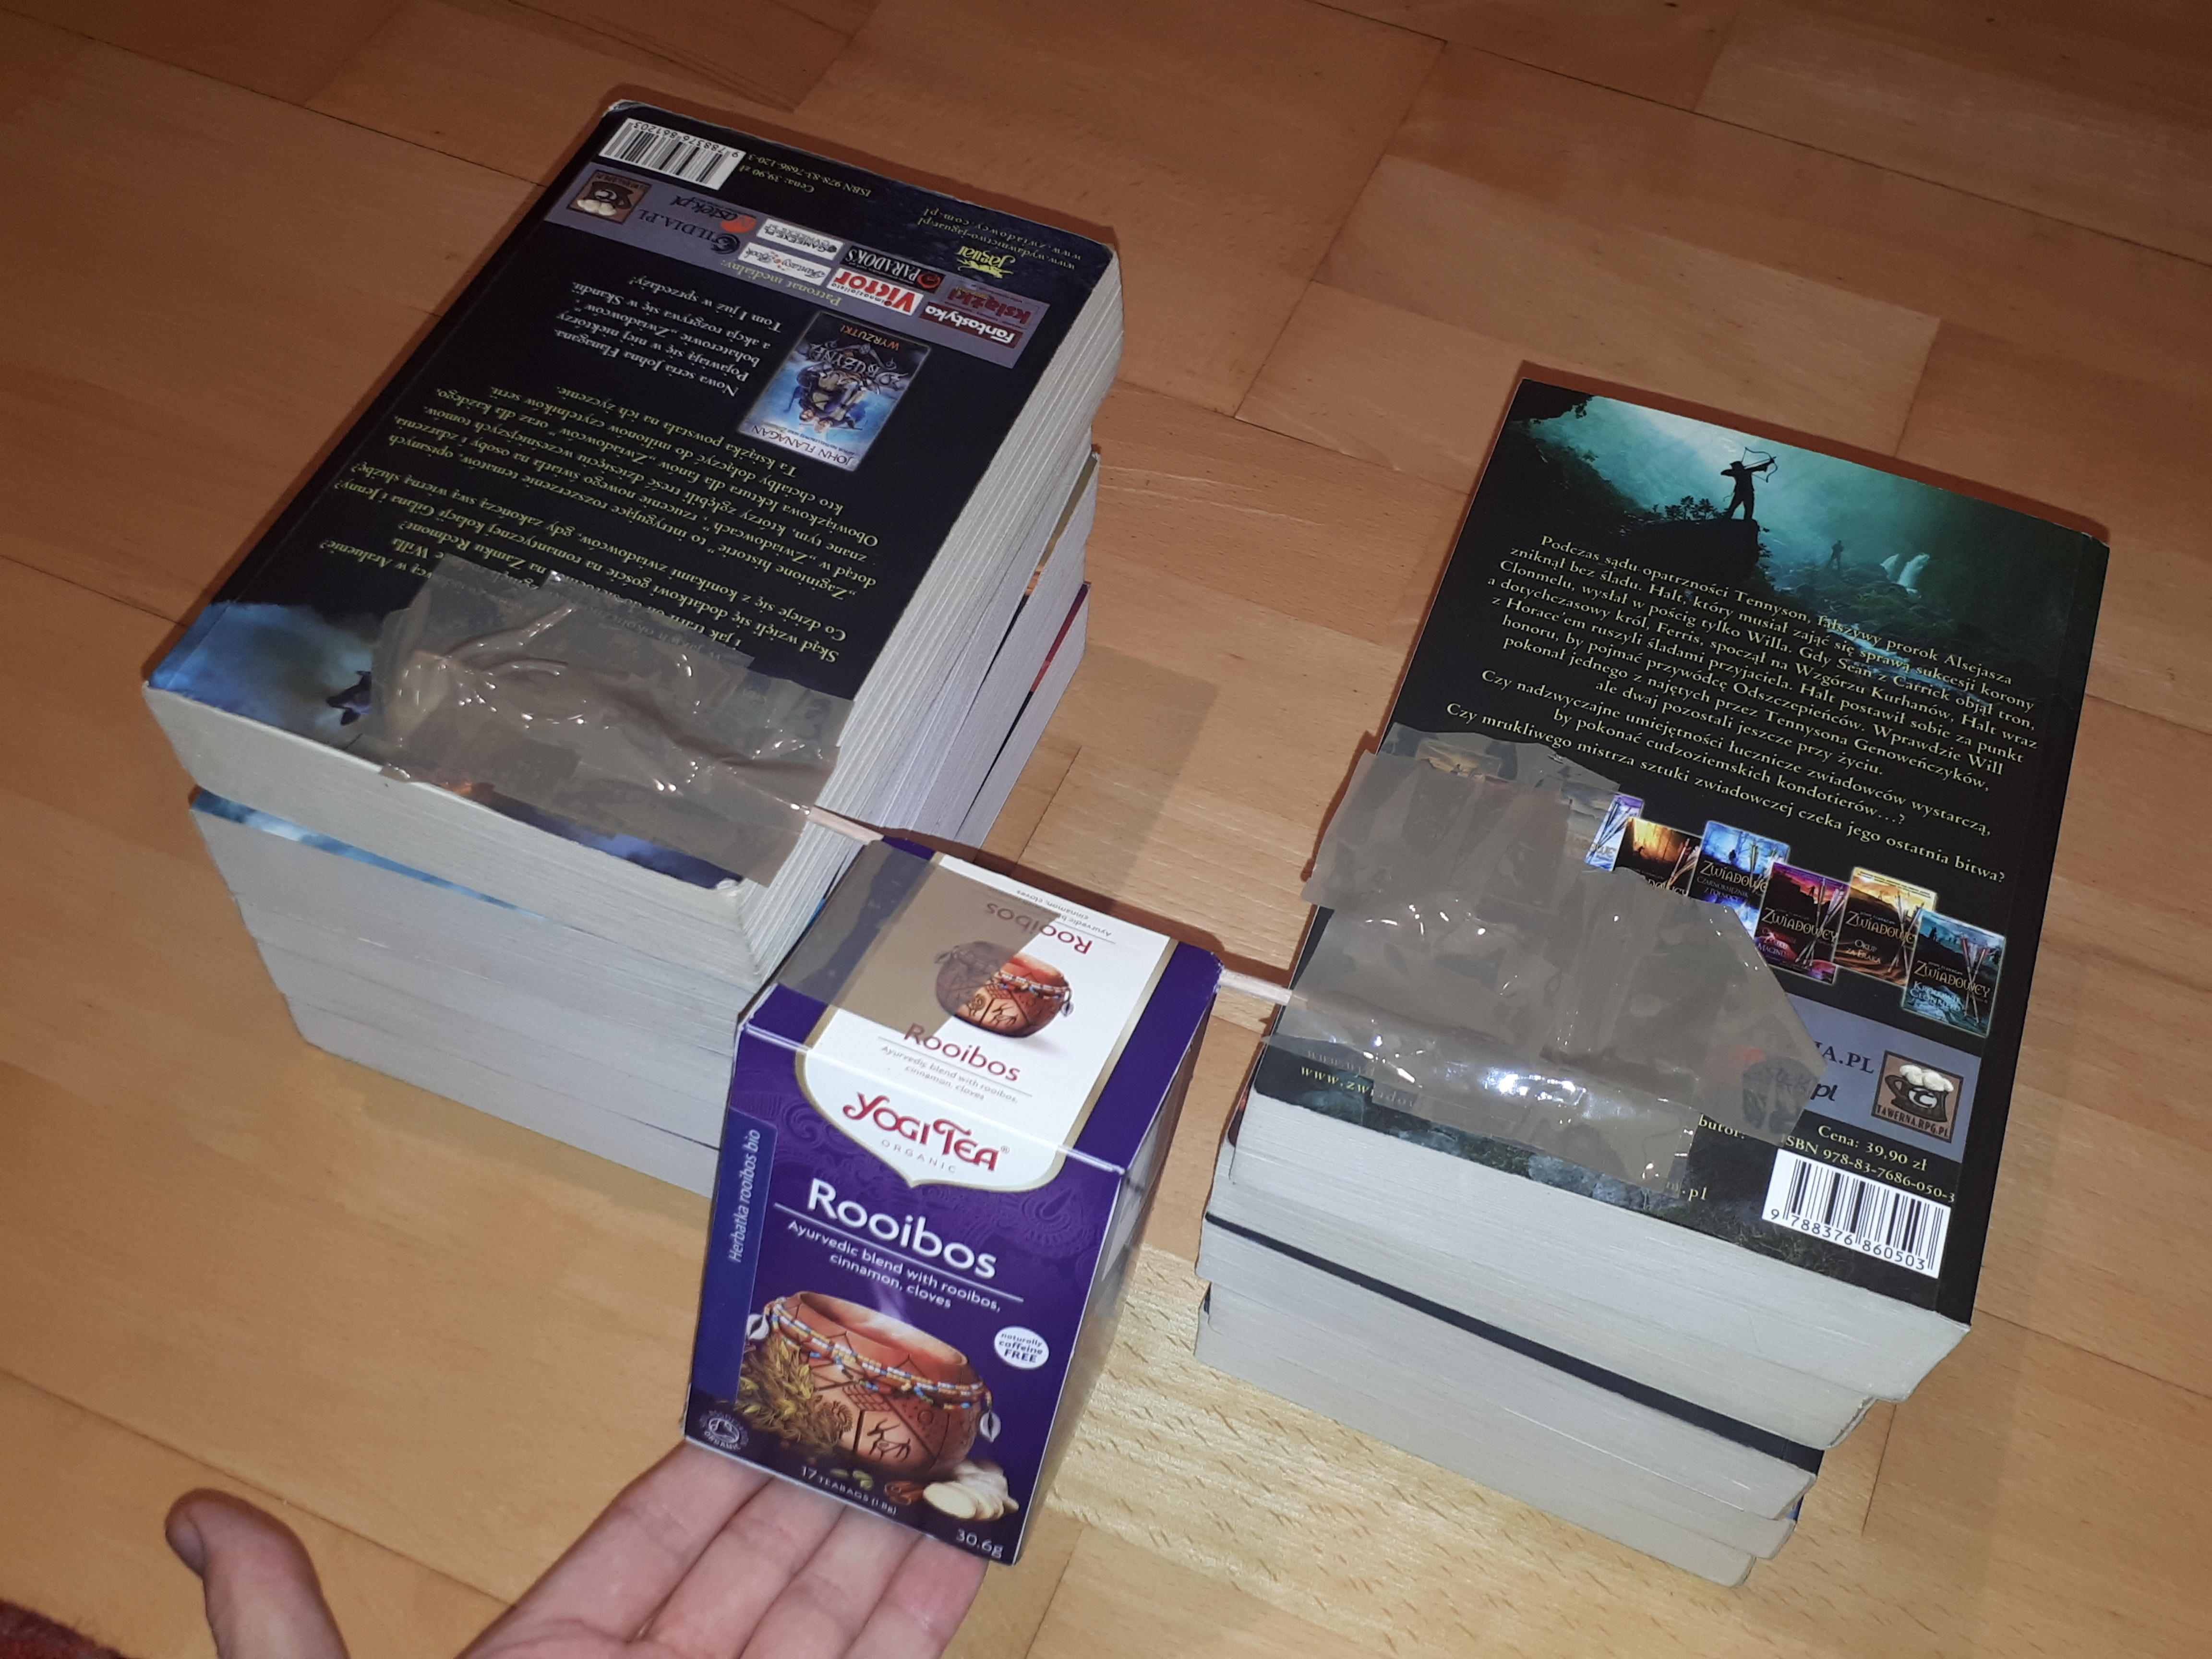
\includegraphics[width=\linewidth]{3}
    \caption{Promień światła biegnący
poniżej powierzchni cieczy }
  \end{subfigure}
  \begin{subfigure}[b]{0.4\linewidth}
    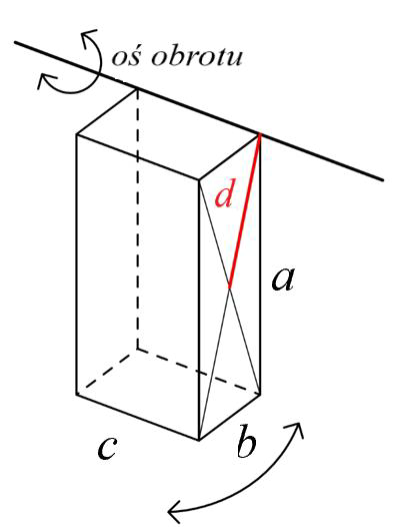
\includegraphics[width=\linewidth]{4}
    \caption{Bieg promienia przez powietrze}
  \end{subfigure}
  
\end{figure}




\section{Przebieg doświadczenia}
 Odmierzoną ilość wody wlaliśmy do czajnika, a następnie uruchomiliśmy go, jednocześnie włączając pomiar na stoperze. Gdy czajnik wyłączył się, zakończyliśmy pomiar czasu. Następnie ostudziliśmy czajnik. Następnie sześciokrotnie powtórzyliśmy powyższą procedurę. Na koniec przeprowadziliśmy odkamienianie czajnika, po czym wykonaliśmy jeden, kontrolny pomiar czasu zagotowania się wody w czajniku.

\newpage

\section{Wyniki Pomiarów}

Producent: Philips\newline
Napięcie zasilania: 220-240 [V]\newline
Moc znamionowa 1850-2200 [W]\newline
Przyjęta moc: 1850 [W]\newline
Pomiar nr. 8 to pomiar po odkamienianiu czajnika


	\begin{table}[H]
		\centering
		\begin{tabular}{|l|l|l|l|l|l|l|l|l|l|}
			\hline
nr & Objetosc [m^3] & T. pocz. [C] & T. końcowa [C] & \Delta T [s] & Cieplo \(Q_{uz}\) [J] & Czas [s] & Sprawność 	\eta [\%] & \(u(\eta) [\%]\)\\ \hline
1 & 0,0005 & 16,6 & 100,0 & 83,4 & 174723 & 113,8 & 83 & 17 \\ \hline
2 & 0,0007 & 21,0 & 100,0 & 79,0 & 231707 & 146,3 & 86 & 13 \\ \hline
3 & 0,0010 & 16,0 & 100,0 & 84,0 & 351960 & 202,5 & 94,1 & 9,5 \\ \hline
4 & 0,0015 & 14,8 & 100,0 & 85,2 & 535482 & 298,1 & 97,1 & 6,5 \\ \hline
5 & 0,0008 & 18,1 & 100,0 & 81,9 & 274528 & 173,7 & 85 & 11 \\ \hline
6 & 0,0013 & 15,1 & 100,0 & 84,9 & 462450 & 267,8 & 93,4 & 7,2 \\ \hline
7 & 0,0012 & 14,0 & 100,0 & 86,0 & 432408 & 259,8 & 90,0 & 7,6 \\ \hline
8 & 0,0010 & 17,0 & 100,0 & 83,0& 347770 & 196,2 & 95,8 & 9,6 \\ \hline
 


		\end{tabular}
		\textbf{\caption{Wyniki pomiarów czasu ogrzewania wody i ilości użytej wody}
		}
	\end{table}

Średnia sprawność siedmiu pomiarów: \(\eta = 90 \%\)
	
\newline


\section{Opracowanie wyników Pomiarów}
    \subsection{Stosowane wzory}
    \[\eta = \frac{m c  _w \Delta T}{tP_{d}}\]
    \subsection{Niepewności}
    \(u_{V}= 0,0001 \:[m^3]\)
    \newline
    \(u_{m}=0,1 \:[kg]\)
    \newline
    \(u_{T}= 0,1 \:[K]\)
    \newline
    \(u_{t}=0,1 \:[s] \)
    \newline
    \(u_{P_{d}}=10 \:[W]\)\newline
    
Niepewność z prawa przenoszenia niepewności:

    \[u(\eta) = \sqrt{(\frac{c_{w}\Delta T u(m)}{tP_{d}})^2 + (\frac{m\Delta T u(c_{w})}{tP_{d}})^2 + (\frac{mc_{w} u(\Delta T)}{tP_{d}})^2 +(\frac{-mc_{w}\Delta T u(t)}{t^2P_{d}})^2 +(\frac{-mc_{w}\Delta T u(P_{d})}{t(P_{d})^2})^2}\]
    \[u(\eta_1)  = 0,166074366 \approx 0,17 = 17  \: [\%]\]
Pozostałe są liczone w taki sam sposób i są w tablice powyżej.\newline
    
    
    
    
Niepewność jako estymator odchylenia:

    \[u(\eta_{sr}) = \sqrt{\frac{\sum (\eta_i - \eta_{śr})^2}{n(n-1)}} = 0,018879764 \approx 0,019 = 1,9 \: [\%]\]

    \subsection{Sprawność po odkamienianiu}
Sprawność po odkamieniu wraz z niepewnością:
\[\eta_8 = 95,8 \: [\%]\]
\[u_{\eta_8} = 0,095943426 \approx 0,096 = 9,6\:[\%]\]

Średnia sprawność siedmiu pomiarów: \(  \eta = 90 \%\)

\[U(\eta_{8}-\eta_{sr})=k\sqrt{[u(\eta_{sr})^2 + u(\eta_{8})^2} = 2\sqrt{(0,1)^2-(0,096)^2}=0,056=5,6 \:[\%]\]

\[\eta_{8}-\eta_{sr}=|0,958-0,9|=0,58=5,8\:[\%] > 5,6\:[\%] \]


 



\subsection{Wnioski}
\begin{itemize}
		\item 
		\item 
		\item Niepewność \(\eta\) obliczona z prawa przenoszenia niepewności jest większa niż niepewność uzyskana jako estymator odchylenia standardowego średniej dla siedmiu pomiarów.
	\end{itemize}
\end{document}